\documentclass{article}

\usepackage[%
    left=0.5in,%
    right=0.5in,%
    top=0.5in,%
    bottom=0.5in,%
]{geometry}%
\usepackage{minitoc}
\usepackage{multicol}
\usepackage{graphicx}
\usepackage{fixltx2e}
\usepackage{listings}
\usepackage{color}
\usepackage{hyperref}
    \hypersetup{ colorlinks = true, linkcolor = blue }
\usepackage{blindtext}
\definecolor{lightgray}{gray}{0.9}
\graphicspath{ {./} }

\newcommand{\inlinecode}[2]{\colorbox{lightgray}{\lstinline
[language=#1]$#2$}}
\newcommand{\worddef}[1]{\hyperref[sec:reference]{\textit{#1}}}

\begin{document}

\tableofcontents

\newpage

\section{Application onCreate}

\begin{multicols}{2}
Implementation:
\begin{itemize}
  \item Extending the Application object
  \item Manifest: android:name=“packagename.myapplicationname” 
\end{itemize}
What could be included in the \texttt{onCreate} of Application?
\begin{itemize}
  \item Initialise the required SDK and libraries of your app
  \item Register any dynamic broadcast receivers your app uses
  \item Create and manage any services your app needs 
\end{itemize}
Practices
\begin{itemize}
  \item Provide the flexibility of controlling the entry point and able to respond efficiently at any stage of being invoked.
  \item Do not do any work that may \textbf{block the app} (e.g. create network connection)
  \item \textbf{Never store mutable instance data} inside the Application object, as it is not guaranteed to stay in memory forever, it will get killed.
\end{itemize}

\vfill\null

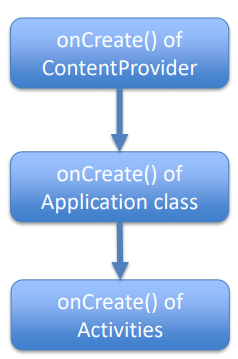
\includegraphics[scale=0.6]{app_oncreate.png}

\end{multicols}

\section{Code Optimisation}

\begin{itemize}
  \item Minimise object creation: Not using temporary objects but use existing object.
  \item Make method static if no need to modify the state of an object.
  \item Make any constants static final
  \item Int is 2x faster than float
\end{itemize}

\section{Application Release}

\begin{itemize}
  \item Remove Logging, disable debugging (i.e. remove android:debuggable in manifest), remove tracing calls
  \item Remove test libraries, frameworks, extra JAR files, unused layouts, strings, etc
  \item Only keep the required <users-permission>
  \item Specify compatibility 
  \item Support library for backward compatibility
\end{itemize}

\pagebreak
\section*{Reference section} \label{sec:reference}
\begin{description}
	\item[placeholder] \hfill \\
\end{description}
\end{document}
